\subsection{Apresentação de Imagens}
A apresentação das imagens é definida em 2 níveis, o nível de pré-visualização, por exemplo, a miniatura da imagem de uma tópico no fórum e o nível do detalhe, onde é possível visualizar a imagem em ponto grande e realizar \textit{zoom}.

Para a apresentação da miniatura da imagem foi decidido apresentar até quatro imagens, sendo que, acima de quatro imagens serão apenas demonstradas três, o que significa que a quarta imagem indicaria quantas mais existem para ser visualizadas. 

Para a implementação da apresentação das miniaturas das imagens utilizou-se a biblioteca \textit{staggered\_grid\_view}, que permite organizar imagens em grelha. Neste contexto desejava-se estruturar as imagens em diferentes aspetos e disposições, pelo que, esta biblioteca permite indicar quantas colunas e linhas existem na grelha ao criar o agrupamento de imagens. Deste modo, decidiu-se que quando são duas imagens, estas dividem a grelha, quando são três imagens, a primeira divide metade da grelha e as outras duas dividem a outra metade, quando são quatro ou mais, as quatro separam a grelha por igual. Quando existem mais do que quatro imagens, optou-se por colocar um filtro de desfoque sobre a última imagem e por cima desta quantas mais imagens existem para apresentar.

\begin{figure}[htb]%
 \centering
 \subfloat[\centering Tópico com 5 imagens]{{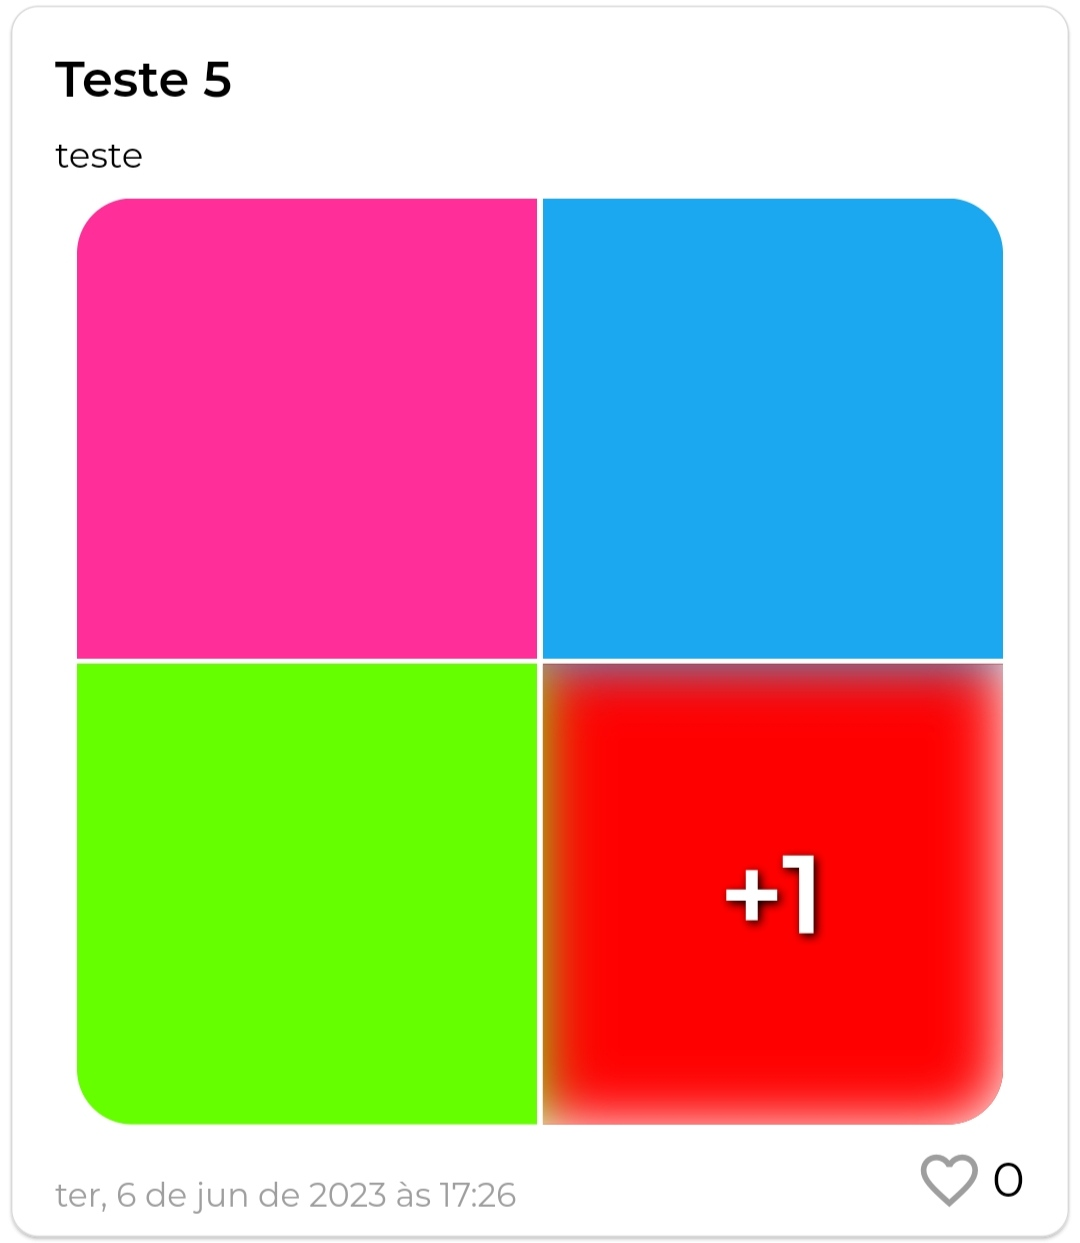
\includegraphics[width=0.25\textwidth]{images/implementacao/frontend/apresentacao_imagens/1686068843028.jpg} }}%
 \qquad
 \subfloat[\centering Tópico com 4 imagens]{{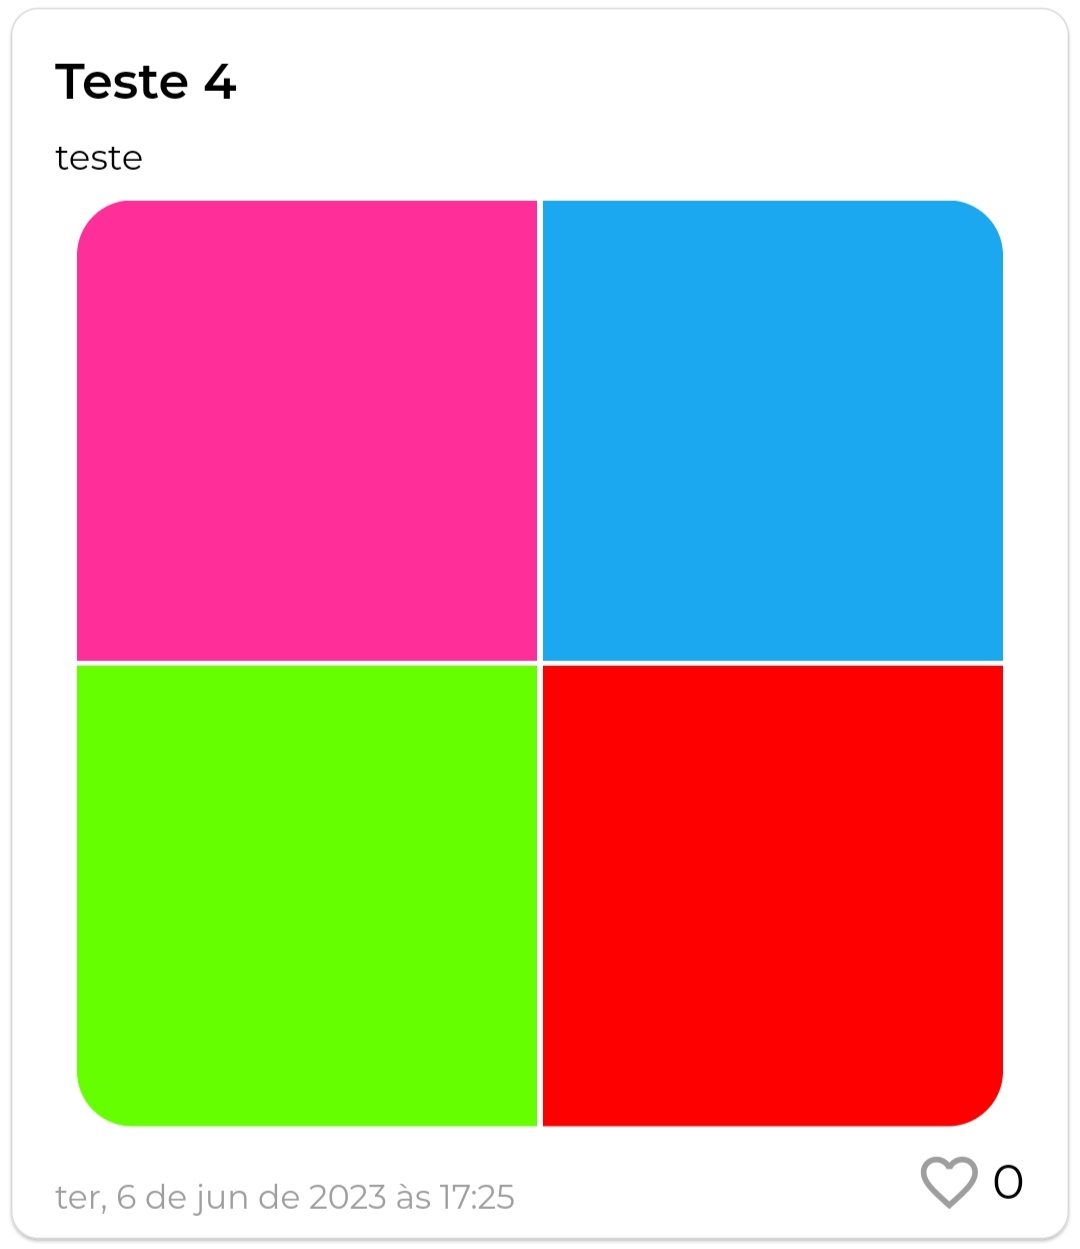
\includegraphics[width=0.25\textwidth]{images/implementacao/frontend/apresentacao_imagens/1686068843039.jpg} }}%
 \qquad
 \subfloat[\centering Tópico com 3 imagens]{{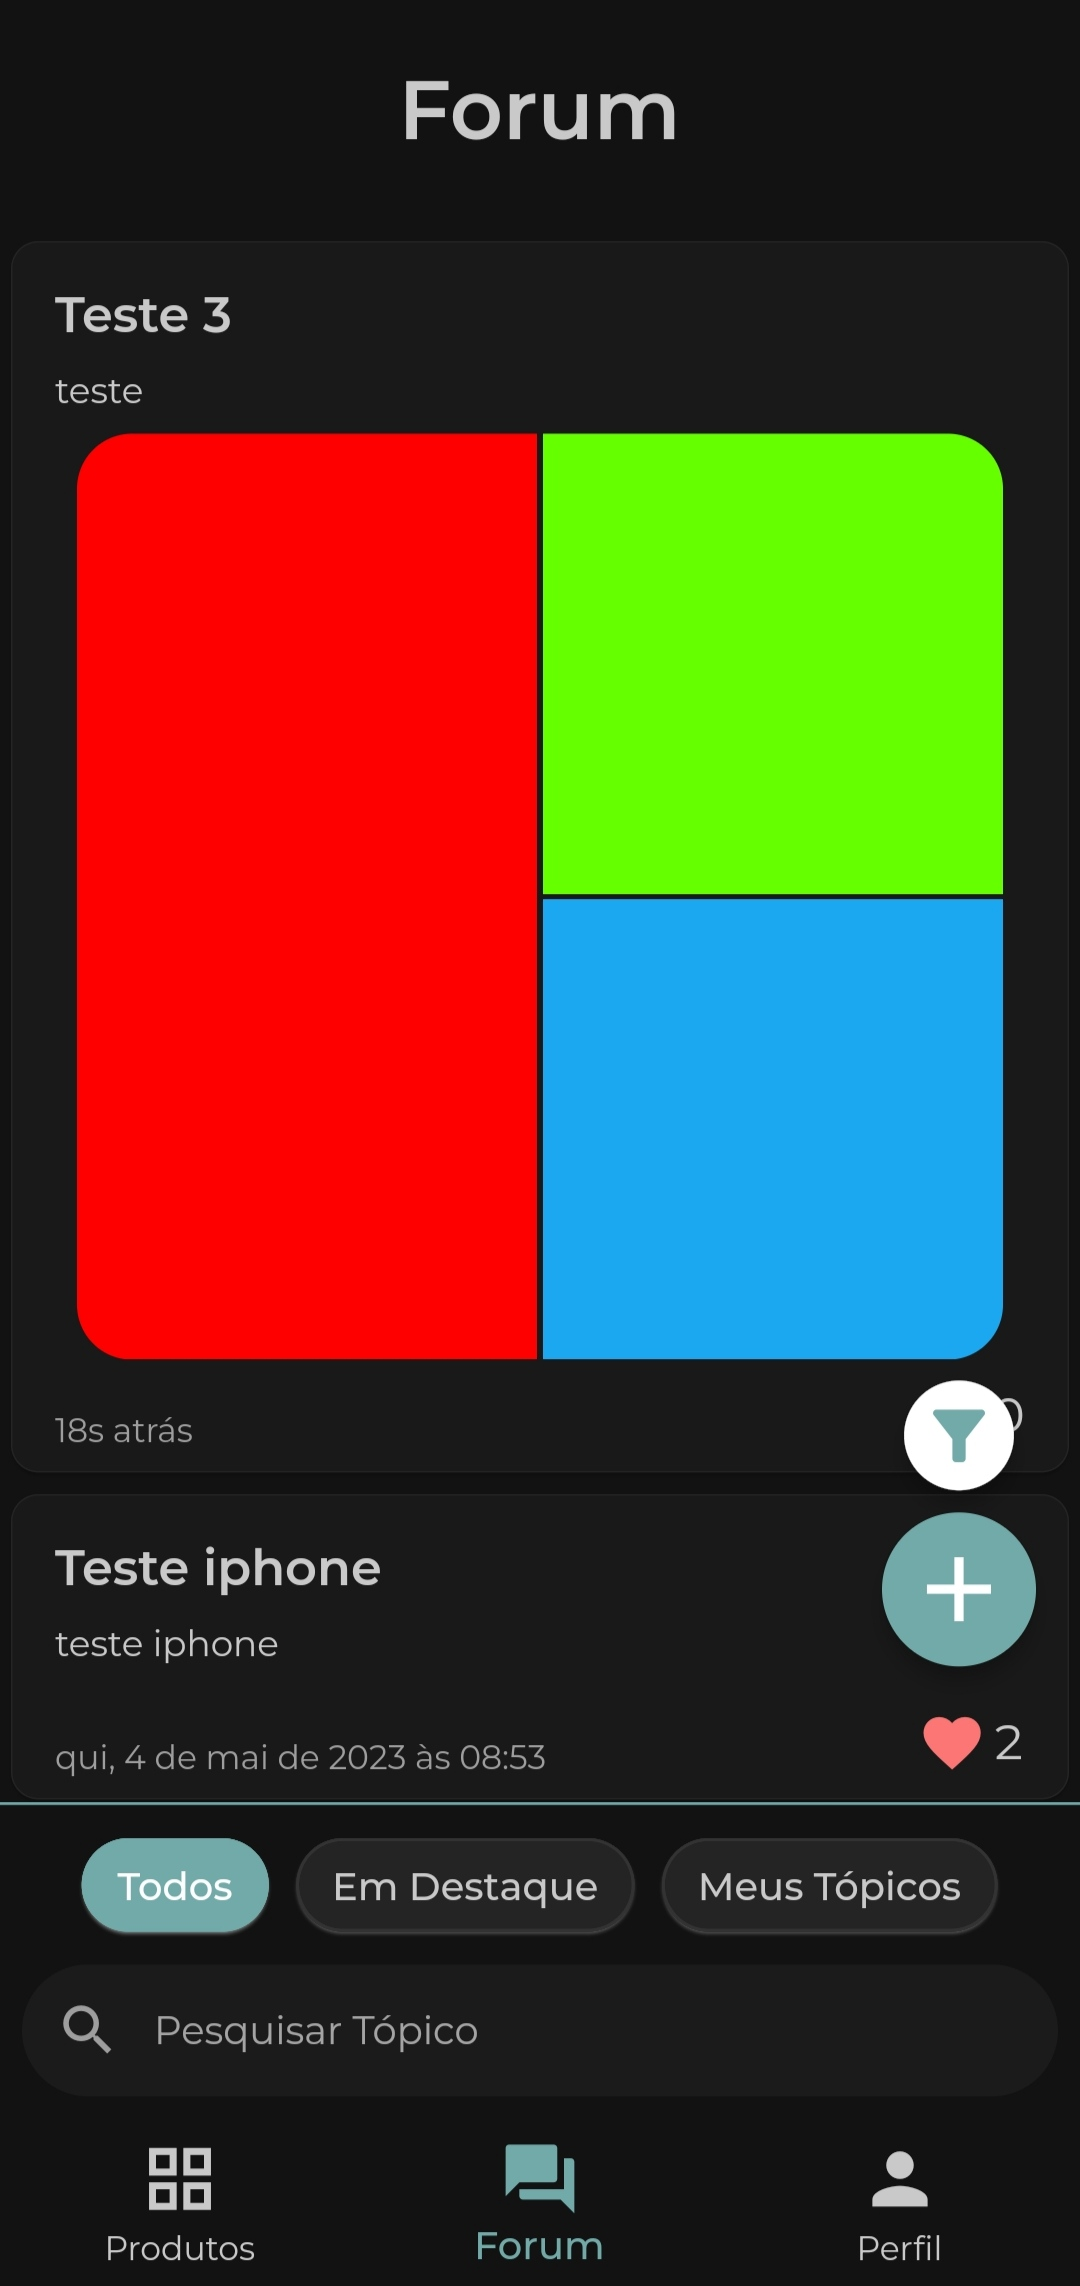
\includegraphics[width=0.25\textwidth]{images/implementacao/frontend/apresentacao_imagens/1686068843051.jpg} }}%
 \qquad
 \subfloat[\centering Tópico com 2 imagens]{{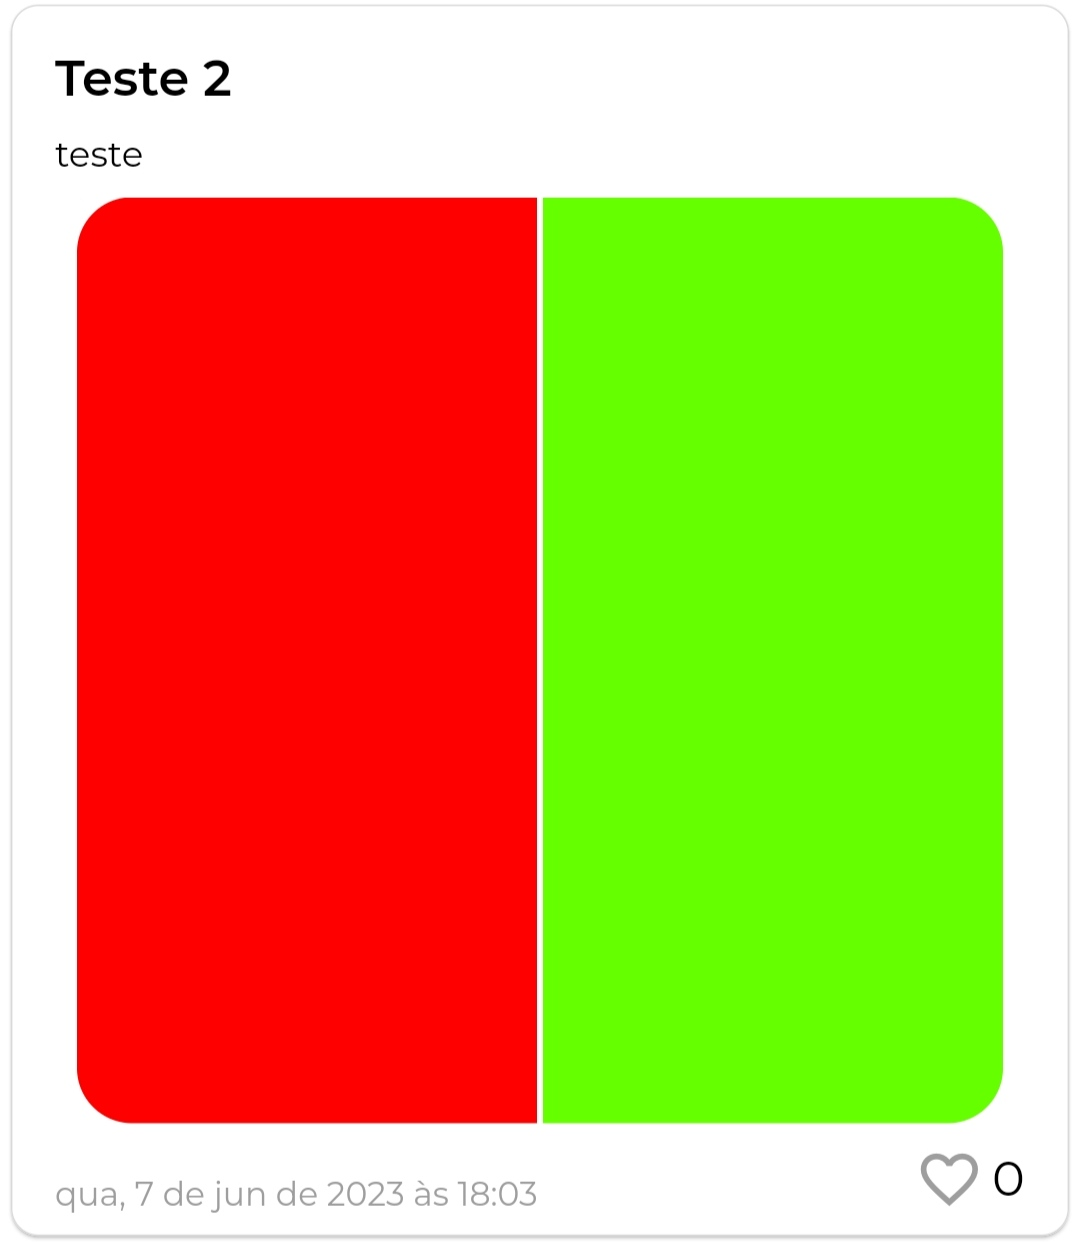
\includegraphics[width=0.25\textwidth]{images/implementacao/frontend/apresentacao_imagens/1686845317274.jpg} }}%
 \qquad
 \subfloat[\centering Tópico com 1 imagem]{{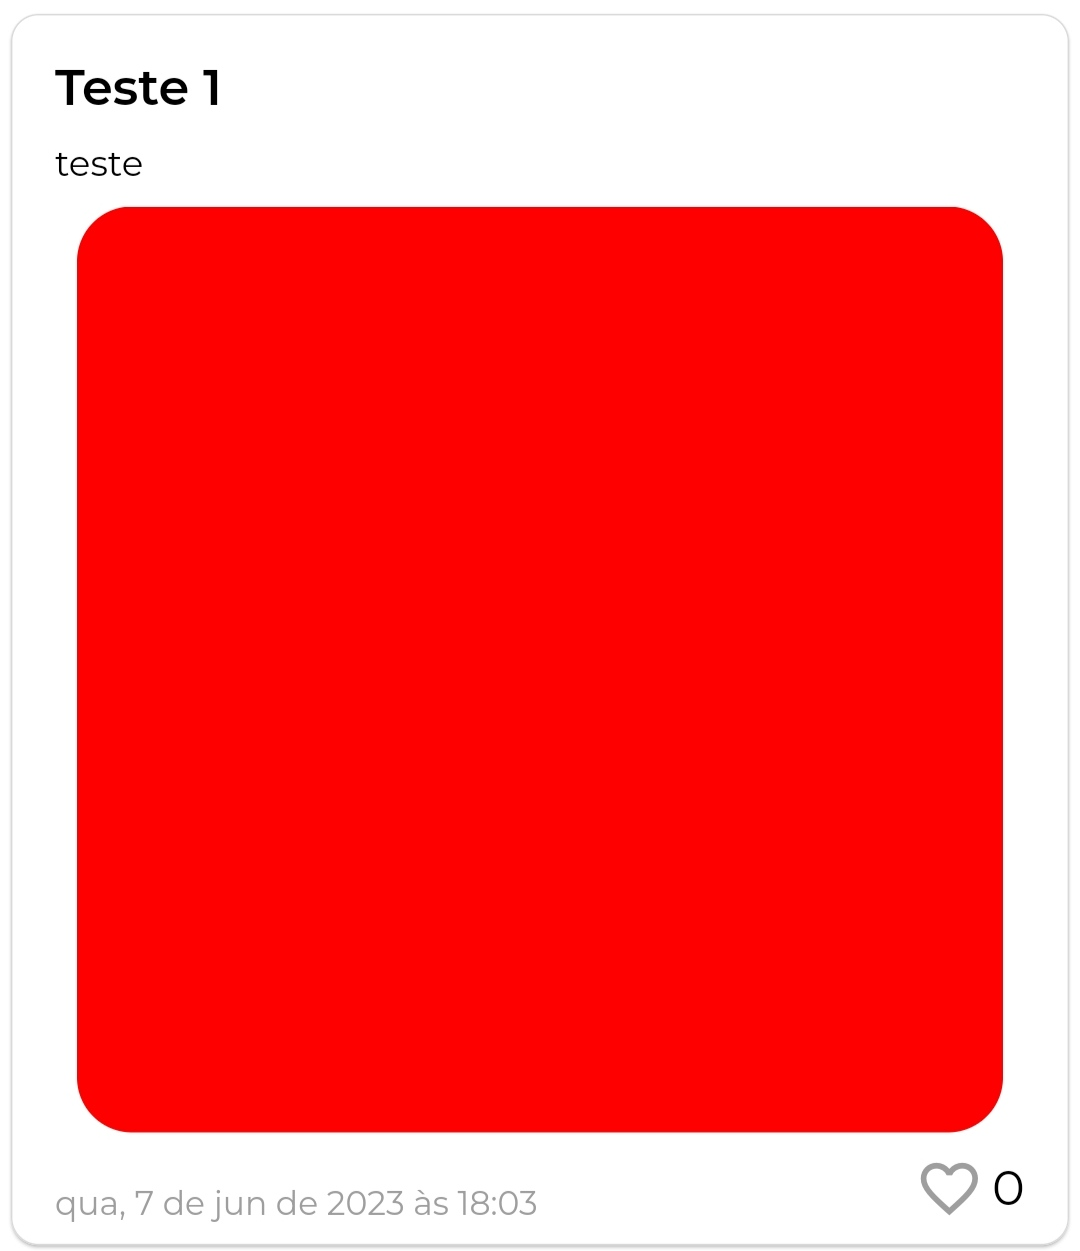
\includegraphics[width=0.25\textwidth]{images/implementacao/frontend/apresentacao_imagens/1686845317288.jpg} }}%
 \label{fig:77}%
\end{figure}

\newpage

\subsection{Apresentação de Imagens em carrosel}

A apresentação das imagens deverá permitir que o utilizador visualize em ponto grande e realize diversas ações sobre estas. Para isso experimentaram-se diversas bibliotecas, mas nunca se alcançou o comportamento desejado, sendo assim, decidiu-se criar o próprio carrossel de imagens, sendo que, o próprio \textit{Flutter} já disponibiliza um \textit{widget} para tal.

O ponto de maior dificuldade para este processo foi a implementação de \textit{zoom}, visto que, o \textit{Flutter} não dispõe de \textit{widgets} para tal. Por isso foi necessário primeiramente detetar gestos com o detetor de gestos da ferramenta e aplicado um \textit{zoom} sobre o centro do gesto. Os gestos aceites foram o de pinça e o gesto de duplo clique.

O grande problema com esta solução é, uma vez que, é permitido um \textit{scroll} horizontal de imagens, os gestos por vezes poderão não funcionar corretamente, principalmente o gesto de pinça que se efetuado na horizontal poderá resultar num \textit{scroll}. Para resolver tal problema definiu-se que quando dois dedos são reconhecidos no ecrã, a navegação horizontal fica bloqueada e, assim que, estes são retirados, a navegação horizontal é ativada novamente.

\subsection{Carregamento de Imagens}

O carregamento de imagens do dispositivo poderá ser realizado por meio da seleção da galeria. Para realizar esta seleção, em primeiro lugar, foi testada a biblioteca \textit{image\_picker}, contudo, esta biblioteca utiliza o seletor de ficheiros do dispositivo. Este seletor de ficheiros permite a seleção de qualquer tipo de ficheiros o que faz com que seja necessário um conjunto de outras verificações, para garantir que apenas as imagens são selecionadas. Isto levaria a uma possível perda do desempenho e da qualidade na experiência de utilização.

Sendo assim, de seguida foi testada a biblioteca \textit{advanced\_image\_picker}, todavia, o problema desta biblioteca é que não permite selecionar vídeos. Posteriormente decidiu-se experimentar a biblioteca \textit{wechat\_asset\_picker}. Esta cria uma página própria para seleção de imagens e vídeos diretamente da galeria. Também permite indicar o limite máximo de seleção e os tipos de ficheiros que o utilizador poderá selecionar, para que apenas, os tipos aceites sejam demonstrados. Por fim, o único ponto desvantajoso é que não é possível traduzir o botão de confirmação da seleção de ficheiros.

Após carregar os ficheiros para a memória, estes são enviados para o \textit{firestorage}.